% Fig 2.9 / spec Fig A05 -- the slope of the cdf is the pdf
% Source: mathstatch2.tex lines 509-552
% F(x) = 2.7 e^{2(x-3)} / (1 + e^{2(x-3)}); upper bound (asymptote) 2.7
% a = 3.9, F(a) = 2.317002, F'(a) = 0.657338 (analytic derivative)
\documentclass[tikz,border=2pt]{standalone}
\usepackage{amsmath}
\usepackage{amssymb}
\usepackage{xcolor}
\usetikzlibrary{arrows.meta}
\newcommand{\sssig}{\scriptscriptstyle}

\definecolor{journalink}{HTML}{1F1C18}
\definecolor{journalmuted}{HTML}{8A7F72}
\definecolor{journalaccent}{HTML}{9C2D2D}

\begin{document}
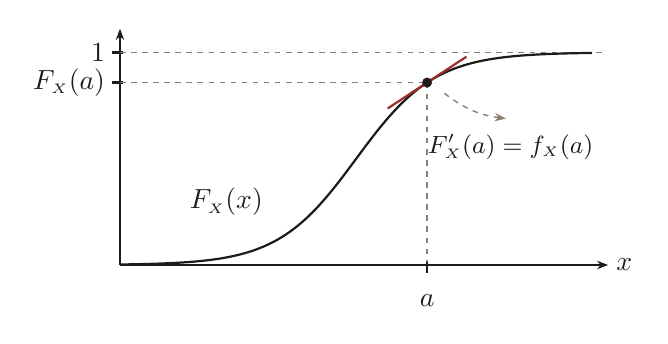
\begin{tikzpicture}[
  x=1cm,
  y=1cm,
  every node/.style={font=\normalsize, journalink},
  axis/.style={journalink, line width=0.8pt, -{Stealth[length=4pt]}},
  tick/.style={journalink, line width=0.8pt},
  guide/.style={journalmuted, line width=0.5pt, dash pattern=on 2pt off 2pt},
  solidpt/.style={circle, fill=journalink, inner sep=0pt, minimum size=3.6pt}
]
  % ---- axes ----
  \draw[axis] (0,0) -- (6.2,0);
  \draw[axis] (0,0) -- (0,3);

  % ---- upper bound (probability 1), redrawn at the true asymptote 2.7 ----
  \draw[tick] (0.035,2.7) -- (-0.106,2.7) node[anchor=east, inner sep=2pt] {$1$};
  \draw[guide] (0,2.7) -- (6.15,2.7);

  % ---- horizontal and vertical guides at a ----
  \draw[tick] (0.035,2.317002) -- (-0.106,2.317002)
    node[anchor=east, inner sep=2pt] {$F_{\sssig X}(a)$};
  \draw[guide] (0,2.317002) -- (3.9,2.317002);
  \draw[guide] (3.9,2.317002) -- (3.9,0);
  \draw[tick] (3.9,0.035) -- (3.9,-0.106);
  \node[anchor=north] at (3.9,-0.25) {$a$};

  % ---- cdf curve ----
  \draw[journalink, line width=0.8pt]
    plot[domain=0:6, samples=200, smooth]
      (\x, {2.7*exp(2*(\x-3))/(1+exp(2*(\x-3)))});

  % ---- tangent line: analytic slope 0.657338, extending 0.5 units either
  %      side of the point of tangency ----
  \draw[journalaccent, line width=0.8pt] (3.4,1.988333) -- (4.4,2.645671);
  \node[solidpt] at (3.9,2.317002) {};

  % ---- pointer arrow (start offset so it does not sit on the guide or curve) ----
  \draw[journalmuted, line width=0.5pt, dash pattern=on 2pt off 2pt,
        -{Stealth[length=4pt]}]
    (4.12,2.18) to[bend right=15] (4.90,1.86);

  % ---- text labels ----
  \node[anchor=east, inner sep=0pt] at (6.02,1.50) {\small $F^{\prime}_{\sssig X}(a) = f_{\sssig X}(a)$};
  \node at (1.35,0.80) {$F_{\sssig X}(x)$};
  \node[anchor=west, inner sep=2.8pt] at (6.2,0) {$x$};
\end{tikzpicture}
\end{document}
